% !TEX encoding = UTF-8 Unicode
% !TEX TS-program = xelatex

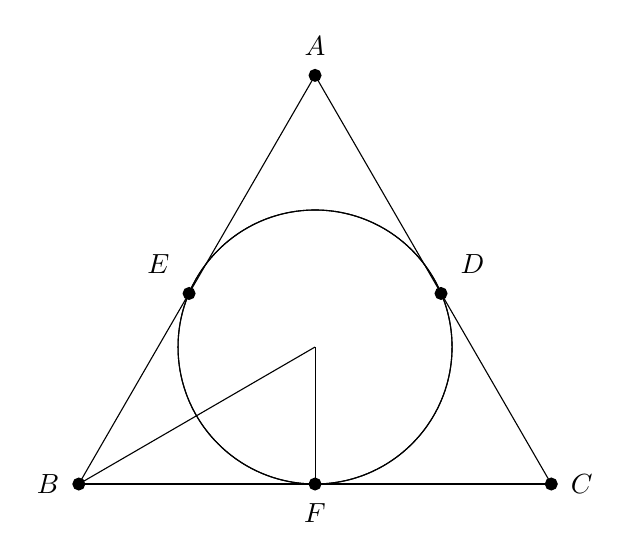
\begin{tikzpicture}
    \coordinate (cBPt) at (0,0);
    \coordinate (cCPt) at (6,0);
    \coordinate (cAPt) at (3.,5.19);
    \coordinate (cEPt) at (1.4,2.42);
    \coordinate (cFPt) at (3,0);
    \coordinate (cDPt) at (4.6,2.42);
    \draw(3.,1.74) circle (1.74);
    \draw (0.,0.)-- (6.,0.);
    \draw (6.,0.)-- (3.,5.19);
    \draw (3.,5.19)-- (0.,0.);
    \draw(3.,1.74) circle (1.74cm);
    \draw (0.,0.)-- (3.,1.74);
    \draw (3.,1.74)-- (3.,0.);
\foreach \v/\u/\t in 
{cAPt/90/$A$,
    cBPt/180/$B$,
    cCPt/0/$C$,
    cDPt/45/$D$,
    cEPt/135/$E$,
    cFPt/270/$F$
}
{
    \draw[ultra thick,fill] (\v) circle (1.5pt);
    \node[label=\u:\t] at (\v){};
};	    

    
\end{tikzpicture}
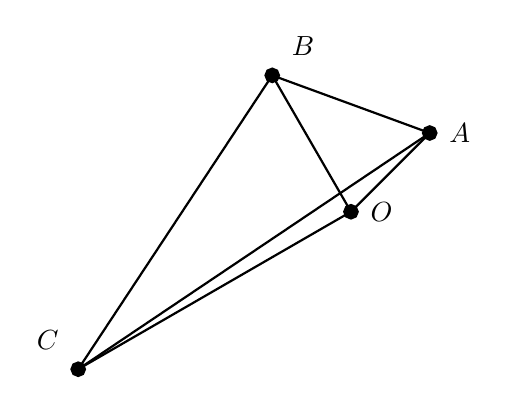
\begin{tikzpicture}
\coordinate (cOPt) at (0,0);
\coordinate (cAPt) at (45:{sqrt(2)});
\coordinate (cBPt) at (120:2);
\coordinate (cCPt) at (210:4);

\foreach \v/\u/\t in 
{cAPt/0/$A$,
    cBPt/45/$B$,
    cCPt/135/$C$,
    cOPt/0/$O$
}
{
    \draw[ultra thick,fill] (\v) circle (2pt);
    \node[label=\u:\t] at (\v){};
};	    

\draw[thick] (cAPt) -- (cBPt) -- (cCPt) circle;
\draw[thick] (cOPt) -- (cAPt) ;
\draw[thick] (cOPt) -- (cBPt) ;
\draw[thick] (cAPt) -- (cCPt) ;
\draw[thick] (cOPt) -- (cCPt) ;


\end{tikzpicture}

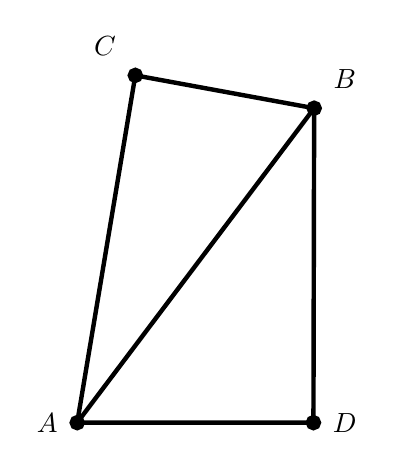
\begin{tikzpicture}

\coordinate (cAPt) at (0,0);
\coordinate (cBPt) at (53:5);
\coordinate (cCPt) at (80.5:{2*sqrt(5)});
\coordinate (cDPt) at (3,0);


\foreach \v/\u/\t in 
{cAPt/180/$A$,
    cBPt/45/$B$,
    cCPt/135/$C$,
    cDPt/0/$D$
}
{
    \draw[ultra thick,fill] (\v) circle (2pt);
    \node[label=\u:\t] at (\v){};
};	    

\draw[ultra thick] (cAPt) -- (cDPt) -- (cBPt)  -- (cCPt) -- (cAPt) circle;
\draw[ultra thick] (cAPt) -- (cBPt) ;

\end{tikzpicture}
